\documentclass[11pt,a4paper,headinclude,footinclude,DIV16,normalheadings]{scrartcl}
%\usepackage[today,nofancy]{svninfo}
\usepackage[automark]{scrpage2}
\usepackage[ansinew]{inputenc}
%\usepackage{german}
%\usepackage{bibgerm}
\usepackage{amsmath}
\usepackage{amsfonts}
\usepackage{theorem}
\usepackage{tikz}
\usepackage{color}
\usepackage{listings}
\lstset{language=bash, basicstyle=\normalfont\ttfamily\scriptsize,
  keywordstyle=\color{black}\bfseries, tabsize=4,
  stringstyle=\ttfamily, commentstyle=\it, extendedchars=true}
\usepackage{hyperref}
\usepackage{makeidx}
\usepackage{xspace}

\usepackage{graphicx}

\newtheorem{lst}{Listing}
\newtheorem{remark}{Remark}[section]

\newcommand{\dune}{\texttt{DUNE}\xspace}
\newcommand{\autoconf}{\texttt{autoconf}\xspace}
\newcommand{\automake}{\texttt{automake}\xspace}
\newcommand{\autogen}{\texttt{dune-autogen}\xspace}
\newcommand{\libtool}{\texttt{libtool}\xspace}
\newcommand{\configure}{\texttt{configure}\xspace}
\newcommand{\configureac}{\texttt{configure.ac}\xspace}
\newcommand{\makefile}{\texttt{Makefile}\xspace}
\newcommand{\makefilein}{\texttt{Makefile.in}\xspace}
\newcommand{\makefileam}{\texttt{Makefile.am}\xspace}
\newcommand{\dunecommon}{\texttt{dune-common}\xspace}
\newcommand{\duneistl}{\texttt{dune-istl}\xspace}
\newcommand{\dunegrid}{\texttt{dune-grid}\xspace}
\newcommand{\dunegridhowto}{\texttt{dune-grid-howto}\xspace}
\newcommand{\dunegriddevhowto}{\texttt{dune-grid-dev-howto}\xspace}
\newcommand{\dunecontrol}{\texttt{dunecontrol}\xspace}
\newcommand{\duneproject}{\texttt{duneproject}\xspace}
\newcommand{\dunemodule}{\texttt{dune.module}\xspace}
\newcommand{\make}{\texttt{make}\xspace}
\newcommand{\topsrc}{\$(top\_srcdir)}

\newcommand{\executable}[1]{{\em #1}\xspace}

\pagestyle{scrheadings}

\title{The DUNE Buildsystem HOWTO}

\author{Christian Engwer$^\ast$ 
% \and Felix Albrecht$^\dagger$
}

%\date{\svnToday}
\date{March 1 2009}

\publishers{%
\vspace{10mm}
{\normalsize $^\ast$Interdisziplin\"ares Zentrum f\"ur Wissenschaftliches Rechnen,
Universit\"at Heidelberg,\\
Im Neuenheimer Feld 368, D-69120 Heidelberg, Germany}\\
%
% \bigskip
% {\normalsize $^\dagger$Institut f\"ur Numerische und Angewandte Mathematik,
% Westf\"alische Wilhelms-Universit\"at M\"unster,\\
% Einsteinstr. 62, D-48149 M\"unster, Germany}\\
% %
\bigskip
{\normalsize \url{http://www.dune-project.org/}}\\
}

\begin{document}

\maketitle
\tableofcontents
\pagebreak

\section{Getting started}\label{section::getting_started}

\textbf{TODO: How do I build the grid howto?}

\section{Creating a new \dune project}\label{section::creating_new_dune_project}

From a build system point of view there is no difference between a \dune
application and a \dune module.

\dune modules are packages that offer a certain functionality that can
be used by \dune applications. Therefore \dune modules offer libraries
and/or header files. A \dune module needs to comply with certain rules
(see~\ref{guidelines}).

Creating a new \dune project has been covered in detail in 
\ref{section::creating_dune_module} using \texttt{duneproject} to take
work off of the user. This is also the recommended way to start a new project. 
If for whatever reasons you do not wish to use \duneproject here is 
the bare minimum you have to provide in order to create a new project:
\begin{itemize}
\item a \dunemodule file\\
  Usually you will only need to specify the parameters \texttt{Module}
  and \texttt{Depends}.
\item \emph{Note:} an \autogen script is \emph{not} needed any more!
\item a basic m4 file\\
  You need to provide two macros \texttt{\emph{MODULE}\_CHECKS}
  and \texttt{\emph{MODULE}\_CHECK\_MODULE} (see~\ref{m4files}).
\item a \configureac file\\
  Have look at the \configureac in \dunegrid for example. The most
  important part is the call to \texttt{DUNE\_CHECK\_ALL} which
  runs all checks needed for a \dune module, plus the checks for the
  dependencies.
\end{itemize}

\subsection{Configuring new \dune module using \duneproject}\label{section::creating_dune_module}

This section tells you how to begin working with \dune without explaining any
further details. For a closer look on \duneproject, see section
\ref{section::creating_new_dune_project}.

Once you have downloaded all the \dune modules you are interested in, you probably
wonder ``How do I start working with \dune?'' It is quite easy.
Let us assume you have a terminal open and are inside a directory containing
some \dune modules. Let us say
 
\begin{lstlisting}[language=make]
ls -l
\end{lstlisting}
produces something like:

\begin{lstlisting}[language=make]
dune-common/
dune-grid/
config.opts
\end{lstlisting}

There is no difference between a \dune module you have downloaded from
the web and modules you created yourself.
\dunecontrol takes care of configuring your project and creating the
correct \texttt{Makefile}s (so you can easily link and use all the other \dune
modules). It can be done by calling
 
\begin{lstlisting}[language=make]
./dune-common/bin/duneproject
\end{lstlisting}

\emph{Note:} In case you are using the unstable version
\dune you should be aware that the build system may change,
just like the source code. Therefore it might be that
\texttt{duneproject} is not up to date with the latest changes.

After calling \duneproject, you have to provide a name for your project
(without whitespace), e.g., \texttt{dune-foo}. 
The prefix \texttt{dune-} is considered good practice, but it is not
mandatory.
You are then asked to provide a
list of all modules the new project should depend on (this will be
something like \dunecommon \dunegrid, etc.). At last, you should provide
the version of your project (e.g., \texttt{0.1}) and your email address.
\duneproject now creates your new project which is a folder with the name of your project,
containing some files needed in order to work with \dune.
In our example,
 
\begin{lstlisting}[language=make]
ls -l dune-foo/
\end{lstlisting}
should produce something like

\begin{lstlisting}[language=make]
configure.ac
dune.module
Makefile.am
README
src
 --> dune-foo.cc
doc
\end{lstlisting}

You can now call \dunecontrol for your new project, as you would for any other \dune module. If you have a \texttt{config.opts}\xspace
file configured to your needs (see e.g. the ``Installation Notes'' on
\url{http://www.dune-project.org}), a simple call of

\begin{lstlisting}[language=make]
./dune-common/bin/dunecontrol --module=dune-foo --opts=config.opts all
\end{lstlisting}
should call \autogen, \configure and \make for your
project and all modules your project depends on first.

\begin{remark}
Always call \dunecontrol from the directory containing \dunecommon.
\end{remark}

You can now  simply run

\begin{lstlisting}[language=make]
./dune-foo/src/dune-foo
\end{lstlisting}
which should produce something like

\begin{lstlisting}[language=make]
Hello World! This is dune-foo.
This is a sequential program.
\end{lstlisting}

If you want your \dune module to be usable by other people your
design should follow a certain structure. A good way to indicate that
your module is set up like the other \dune modules is by naming it
with the prefix \texttt{dune-}\xspace.  Since your module should be
concerned with a certain topic, you should give it a meaningful name
(e.g. \dunegrid is about grids).  You will also see that there are
subfolders \texttt{doc/}\xspace, \texttt{foo/}\xspace and
\texttt{src/}\xspace in \texttt{dune-foo/}\xspace.
\texttt{foo/}\xspace will contain any headers that are of interest to
other users (like the subfolder \texttt{common/}\xspace in
\dunecommon, \texttt{grid/}\xspace in \dunegrid, etc.). Other users
will have to include those files if they want to work with them. Let's
say your project provides some interface implementation in a file
\texttt{foo.hh}\xspace. \duneproject already put this an example file
into the subfolder \texttt{dune/foo/}.

\begin{lstlisting}[language=make]
dune-foo/
-> configure.ac
-> doc/
   -> doxygen/
      -> Doxylocal
      -> Makefile.am
   -> Makefile.am
-> dune.module
-> dune/
   -> foo/
      -> foo.hh
      -> Makefile.am
   -> Makefile.am
-> Makefile.am
-> README
-> src/
   -> dune_foo.cc
\end{lstlisting}

After running
\begin{lstlisting}[language=make]
make doc
\end{lstlisting}
in \texttt{dune-foo} you should now find a
\texttt{html} \texttt{doxygen} documentation which can be read by opening
\texttt{dune-foo/doc/doxygen/html/index.html}.

\section{Dune module guidelines}\label{section::dune_module_guidelines}
\label{guidelines}

A \dune module should comply with the following rules:
\begin{itemize}
\item Documentation is located under \texttt{doc/} and gets
  web-installed under \texttt{BASEDIR/doc/}.
\item \automake includes are located in \dunecommon. To use them, you
  will have to make a symbolic link to \texttt{dune-common/am/} (see
  \ref{am_includes}). The symlink creation should be handled by the
  \autogen (see~\ref{autogen}).
\item The \texttt{am/} directory does not get included in the tarball.
\item Additional configure tests are located in the \texttt{m4/}
  directory. You should at least provide the macros \texttt{\emph{MODULE}\_CHECKS}
  and \texttt{\emph{MODULE}\_CHECK\_MODULE}, in order to setup and
  find your module (see~\ref{m4files}).
\item Header files should be accessible via \verb!#include <dune/foo/bar.hh>!,
  otherwise they cannot be used by other \dune modules.   When running
  \texttt{make install} all header files should be installed into
  \texttt{\textit{prefix}/include/dune/}.
\end{itemize}

\section{The Structure of \dune}
\dune consists of several independent modules:
\begin{itemize}
\item \dunecommon
\item \dunegrid
\item \duneistl
\item \dunegridhowto
\item \dunegriddevhowto
\end{itemize}

Single modules can depend on other modules and so the \dune modules
form a dependency graph.  The build system has to track and resolve
these inter-module dependencies.

The build system is structured as follows:
\begin{itemize}
\item Each module is built using the GNU AutoTools.
\item Each module has a set of modules it depends on, these modules
  have to be built before building the module itself.
\item Each module has a file \dunemodule which holds dependencies and
  other information regarding the module.
\item The modules can be built in the appropriate order using the
  \dunecontrol script (shipped with \dunecommon)
\end{itemize}

The reasons to use the GNU AutoTools for \dune were the following
\begin{itemize}
\item We need platform independent build.
\item Enabling or disabling of certain features depending on
  features present on the system.
\item Creations of libraries on all platforms.
\item Easy creation of portable but flexible Makefiles.
\end{itemize}

The reasons to add the \dunecontrol script and the \dunemodule
description files were
\begin{itemize}
\item One tool to setup all modules (the AutoTools can only work on one
  module).
\item Automatic dependency tracking.
\item Automatic collection of command-line parameters (\configure needs
  special command-line parameters for all modules it uses)
\end{itemize}

\section{Building Single Modules Using the GNU AutoTools}

Software is generally developed to be used on multiple
platforms. Since each of these platforms has different compilers,
different header files, there is a need to write makefiles and build
scripts that work on a variety of platforms. The Free
Software Foundation (FSF), faced with this problem, devised a
set of tools to generate makefiles and build scripts that work on a
variety of platforms. These are the GNU AutoTools. 
If you have downloaded and built any GNU
software from source, you are familiar with the \configure script. The
\configure script runs a series of tests to get information about
your machine.

The autotools simplify the generation of portable Makefiles and
configure scripts.

\minisec{autoconf}

\autoconf is used to create the \configure script. \configure is
created from \configureac, using a set of \texttt{m4} files.

\begin{center}
  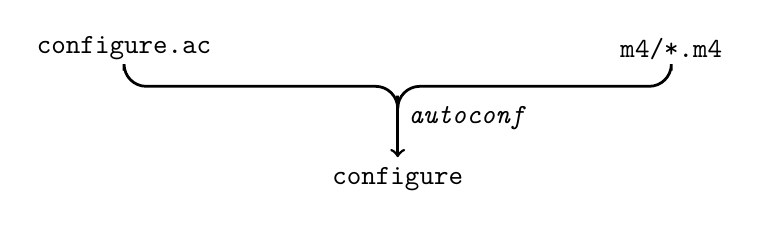
\begin{tikzpicture}[scale=0.05,line width=1pt,rounded corners=8pt]
    \draw (-2,2) node [anchor=south] {\configureac}
          -- (-2,-2) -- (67.5,-2) -- (67.5,-6);
    \draw (137,2) node [anchor=south] {\tt{}m4/*.m4}
          -- (137,-2) -- (67.5,-2) -- (67.5,-6);
    \draw[->] (67.5,-5.5)
          -- (67.5,-10) node [anchor=west] {\textit{\autoconf}}
          -- (67.5,-20) node [anchor=north] {\configure};
  \end{tikzpicture}
\end{center}

How to write a \configureac for \dune is described in Sec.\,\ref{configure.ac}.

\minisec{automake}

\automake is used to create the \makefilein files (needed for
\configure) from \makefileam files, using a set of include files
located in a directory called \texttt{am}. These include files provide
additional features not provided by the standard \automake (see
Sec.\,\ref{am_includes}). The \texttt{am} directory is in the \dunecommon
module and each module intending to use one of these includes has to
have a symlink \texttt{am} that points to \texttt{dune-common/am}.
This link is usually created by \autogen (see Sec.\,\ref{autogen}).

\begin{center}
  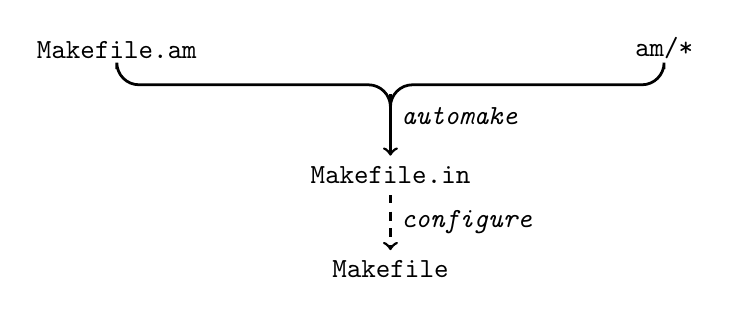
\begin{tikzpicture}[scale=0.05,line width=1pt,rounded corners=8pt]
    \draw (-2,2) node [anchor=south] {\makefileam}
          -- (-2,-2) -- (67.5,-2) -- (67.5,-6);
    \draw (137,2) node [anchor=south] {\tt{}am/*}
          -- (137,-2) -- (67.5,-2) -- (67.5,-6);
    \draw[->] (67.5,-5.5)
          -- (67.5,-10) node [anchor=west] {\textit{\automake}}
          -- (67.5,-20) node [anchor=north] {\texttt{Makefile.in}};
    \draw[dashed, ->] (67.5,-30)
          -- (67.5,-37) node [anchor=west] {\textit{\configure}}
          -- (67.5,-44) node [anchor=north] {\texttt{Makefile}};
  \end{tikzpicture}
\end{center}

Information on writing a \makefileam is described in \ref{makefile.am}

\minisec{libtool}
\libtool is a wrapper around the compiler and
linker. It offers a generic interface for creating static and shared
libraries, regardless of the platform it is running on.

\libtool hides all the platform specific aspects of library creation
and library usage. When linking a library or an executable you (or
\automake) can call the compiler via \libtool. \libtool will then take
care of
\begin{itemize}
\item platform specific command-line parameters for the linker,
\item library dependencies.
\end{itemize}

\minisec{configure}
\label{configure}
\configure will run the set of tests specified in your \configureac.
Using the results of these tests configure can check that all
necessary features (libraries, programs, etc.) are present and can activate
and deactivate certain features of the module depending on what is
available on your system.

For example \configure in \dunegrid will search for the ALUGrid
library and  enable or disable \texttt{Dune::ALU3dGrid}.
This is done by writing a preprocessor macro \verb!#define HAVE_ALUGRID!
in the \texttt{config.h}
header file. A header file can then use an \verb!#ifdef! statement to
disable parts of the code that do not work without a certain
feature. This can be used in the applications as well as in the headers
of a \dune module.

The \texttt{config.h} file is created by \configure from a
\texttt{config.h.in} file, which is automatically created from the
list of tests used in the \configureac.

\subsection{Makefile.am}
\label{makefile.am}

\subsubsection{Overview}

Let's start off with a simple program \executable{hello} built from
\texttt{hello.c}. As \automake is designed to build and install a
package it needs to know

\begin{itemize}
\item what programs it should build,
\item where to put them when installing,
\item which sources to use.
\end{itemize}

The core of a \makefileam thus looks like this:

\begin{lstlisting}[language=make]
noinst_PROGRAMS = hello
hello_SOURCES = hello.c
\end{lstlisting}

This would build \executable{hello} but not install it when \texttt{make
  install} is called. Using \verb!bin_PROGRAMS! instead of
\verb!noinst_PROGRAMS! would install the \executable{hello}-binary into a
\texttt{\textit{prefix}/bin} directory.

Building more programs with several source files works like this

\begin{lstlisting}[language=make]
noinst_PROGRAMS = hello bye

hello_SOURCES = common.c common.h hello.c
bye_SOURCES = common.c common.h bye.c parser.y lexer.l
\end{lstlisting}

\automake has more integrated rules than the standard make, the example
above would automatically use yacc/lex to create
\texttt{parser.c/lexer.c} and build them into the {\em bye} binary.

Make-Variables may be defined and used as usual:

\begin{lstlisting}[language=make]
noinst_PROGRAMS = hello bye

COMMON = common.c common.h

hello_SOURCES = $(COMMON) hello.c
bye_SOURCES = $(COMMON) bye.c parser.y lexer.l
\end{lstlisting}

Even normal make-rules may be used in a \makefileam.

\minisec{Using flags}

Compiler/linker/preprocessor-flags can be set either globally:

\begin{lstlisting}[language=make]
noinst_PROGRAMS = hello bye

AM_CPPFLAGS = -DDEBUG

hello_SOURCES = hello.c
bye_SOURCES = bye.c
\end{lstlisting}

or locally:

\begin{lstlisting}[language=make]
noinst_PROGRAMS = hello bye

hello_SOURCES = hello.c
hello_CPPFLAGS = -DHELLO

bye_SOURCES = bye.c
bye_CPPFLAGS = -DBYE
\end{lstlisting}

The local setting overrides the global one, thus

\begin{lstlisting}[language=make]
hello_CPPFLAGS = $(AM_CPPFLAGS) -Dmyflags
\end{lstlisting}
%$\end{lstlisting}

may be a good idea.

It is even possible to compile the same sources with different flags:

\begin{lstlisting}[language=make]
noinst_PROGRAMS = hello bye

hello_SOURCES = generic-greeting.c
hello_CPPFLAGS = -DHELLO

bye_SOURCES = generic-greeting.c
bye_CPPFLAGS = -DBYE
\end{lstlisting}

Perhaps you're wondering why the above examples used
\texttt{AM\_CPPFLAGS} instead of normal \texttt{CPPFLAGS}? The
reason for this is that the variables \texttt{CFLAGS},
\texttt{CPPFLAGS}, \texttt{CXXFLAGS} etc. are considered {\em user
  variables} which may be set on the command line:

\begin{lstlisting}[language=make]
make CXXFLAGS="-O2000"
\end{lstlisting}

This would override any settings in Makefile.am which might be
necessary to build. Thus, if the variables should be set even if the
user wishes to modify the values, you should use the \texttt{AM\_*}
version. 

The real compile-command always uses both \texttt{AM\_\textit{VAR}} and
\texttt{\textit{VAR}} (or \texttt{\texttt{progname}\_\textit{VAR}} and
\texttt{\textit{VAR}}).  Options that
autoconf finds are stored in the user variables (so that they may be
overridden).

Besides the three types of variables mentioned so far (user-, automake- and
program-variables) there exists a fourth type by convention: variables of
dependent libraries.  These variables have the form
\texttt{\textit{LIBRARY}\_\textit{VAR}} and contain flags necessary to build
programs or libraries which depend on that library.  They are usually included
in \texttt{\textit{program}\_\textit{VAR}}, like this:
\begin{lstlisting}[language=make]
foo_CPPFLAGS = $(AM_CPPFLAGS) $(SUPERLU_CPPFLAGS)
\end{lstlisting}
If all programs build by the same makefile depend on a library,
\texttt{\textit{program}\_\textit{VAR}} can be included in
\texttt{AM\_\textit{VAR}} instead:
\begin{lstlisting}[language=make]
AM_CPPFLAGS = @AM_CPPFLAGS@ $(SUPERLU_CPPFLAGS)
\end{lstlisting}
%$\end{lstlisting}

There are five classes of variables in automake-generated makefiles:
\begin{description}
\item[automake] Example: \texttt{AM\_CPPFLAGS}.  These variables are usually
  undefined by default and the developer may assign them default values in the
  \texttt{Makefile.am}:
  \begin{lstlisting}[language=make]
AM_CPPFLAGS = -DMY_DIR=`pwd`
  \end{lstlisting}
  {\bf Automake} variables are not automatically substituted by
  \texttt{configure}, though it is common for the developer to
  \lstinline[language=make]{AC_SUBST} them.  In this case a different
  technique must be  used to assign values to them, or the substituted value
  will be ignored.  See the {\bf configure-substituted} class below.  The
  names of {\bf automake} variables begin with \texttt{AM\_} most of the time,
  but there are some variables which don't have that prefix.  These variables
  give defaults for {\bf target-specific} variables.
\item[configure-substituted] Example: \lstinline[language=make]{srcdir}.
  Anything can be made a {\bf configure-substituted} variable by calling
  \lstinline[language=sh]{AC_SUBST} in \texttt{configure.ac}.  Some
  variables always substituted by autoconf\footnote{autoconf manual, section
    ``Preset Output Variables''} or automake, others are only substituted when
  certain autoconf macros are used.  In Dune, it is quiet common to substitute
  {\bf automake} variables:
  \begin{lstlisting}[language=sh]
AC_SUBST(AM_CPPFLAGS, $DUNE_CPPFLAGS)
  \end{lstlisting}
  %$\end{lstlisting}
  The value substituted by \texttt{configure} can be augmented in the
  \texttt{Makefile.am} like this:
  \begin{lstlisting}[language=make]
AM_CPPFLAGS = @AM_CPPFLAGS@ -DMY_DIR=`pwd`
  \end{lstlisting}
\item[target-specific] Example: \texttt{\textit{target}\_CPPFLAGS}.  The names
  of these variables are of the form canonical target name followed by an
  underscore followed some uppercase letters.  If there is a {\bf automake}
  variable corresponding to this {\bf target-specific} variable, the uppercase
  letters at the end of the name usually correspond to the name of that {\bf
    automake} variable.  These variables provide target-specific information.
  They are defined by the developer in the \texttt{Makefile.am} and are
  documented in the automake manual.  If there is corresponding a {\bf
    automake} variable it provides a default which is used when the {\bf
    target-specific} variable is not defined.  Example definition:
  \begin{lstlisting}[language=make]
false_SOURCES = true.c
false_CPPFLAGS = $(AM_CPPFLAGS) -DEXIT_CODE=1
  \end{lstlisting}
  %$\end{lstlisting}
  This example also shows how to include the value of the corresponding {\bf
    automake} variable.
\item[user] Example: \texttt{CPPFLAGS}.  These variables are for the user to
  set on the make command line:
  \begin{lstlisting}[language=sh]
make CPPFLAGS=-DNDEBUG
  \end{lstlisting}
  They usually augment some {\bf target-specific} or {\bf makefile-default}
  variable in the build rules.  Often these variables are {\em
    precious}\footnote{autoconf manual,
    \lstinline[language=sh]{AC_ARG_VAR}}, and the user can tell
  \texttt{configure} what values these variables should have.  These variables
  are {\bf configure-substituted}.

  The developer should never set this
  variables in the \texttt{Makefile.am}, because that would override the
  user-provided values given to configure.  Instead, \texttt{configure.ac}
  must be tweaked to set a different default if the user does not give a value
  to \texttt{configure}.
\item[external-library] Example: \texttt{\textit{LIB}CPPFLAGS}.  These
  variables contain settings needed when using external libraries in a
  target.  They should be included in the value for the corresponding {\bf
    target-specific} variable
  \begin{lstlisting}[language=make]
testprog_CPPFLAGS = $(AM_CPPFLAGS) $(SUPERLUCPPFLAGS)
  \end{lstlisting}
  or the {\bf makefile-default} variable
  \begin{lstlisting}[language=make]
AM_CPPFLAGS = @AM_CPPFLAGS@ $(SUPERLUCPPFLAGS)
  \end{lstlisting}
  %$\end{lstlisting}
  Values for these variables are determined by \texttt{configure}, thus they
  are {\bf configure-substituted}.  Usually,
  \texttt{configure.ac} must call the right autoconf macro to determine these
  variables.

  Note that the variable name with an underscore
  \texttt{\textit{LIB}\_CPPFLAGS} is not recommended\footnote{Autoconf
    manual, section ``Flag Variables Ordering''}, although this pattern is
  common.
\end{description}

Commonly used variables are:
\begin{description}
\item[preprocessor flags] These flags are passed in any build rule that calls
  the preprocessor.  If there is a {\bf target-specific} variable
  \texttt{\textit{target}\_CPPFLAGS} defined, the flags are given by
\begin{lstlisting}[language=make]
$(DEFS) $(DEFAULT_INCLUDES) $(INCLUDES) $(target_CPPFLAGS) $(CPPFLAGS)
\end{lstlisting}
  %$\end{lstlisting}
  otherwise
\begin{lstlisting}[language=make]
$(DEFS) $(DEFAULT_INCLUDES) $(INCLUDES) $(AM_CPPFLAGS) $(CPPFLAGS)
\end{lstlisting}
  %$\end{lstlisting}
  is used.
  \begin{description}
  \item[\texttt{DEFS}] Class: {\bf configure-substituted}.  Contains all the
    preprocessor defines from \lstinline[language=sh]{AC_DEFINE} and friends.
    If a \texttt{config.h} header is used, contains just the value
    \texttt{-DHAVE\_CONFIG\_H} instead.
  \item[\texttt{DEFAULT\_INCLUDES}] Class: {\bf configure-substituted}.  This
    variables contains a set of default include paths: \texttt{-I.},
    \texttt{-I\$(srcdir)}, and an path to the directory of \texttt{config.h},
    if that is used.
  \item[\texttt{INCLUDES}] Class: {\bf automake}.  This is an obsolete
    alternative to \texttt{AM\_CPPFLAGS}.  Use that instead.
  \item[\texttt{\textit{target}\_CPPFLAGS}] Class: {\bf target-specific}.
    Target-specific preprocessor flags.  If this variable exists, it overrides
    \texttt{AM\_CPPFLAGS} and causes the renaming of object
    files\footnote{automake manual, ``Why are object files sometimes
      renamed?''}.
  \item[\texttt{AM\_CPPFLAGS}] Class: {\bf automake}.  This is the makefile
    default for any preprocessor flags.
  \item[\texttt{CPPFLAGS}] Class: {\bf user}, {\bf configure-substituted}.
    Flags given by the user, either to \texttt{configure} or when invoking
    \texttt{make}.  If the user didn't provide any value to
    \texttt{configure}, it may contain debugging and optimization options per
    default (like \texttt{-DNDEBUG}).  The value of \texttt{CPPFLAGS} always
    appears after the other preprocessor flags.
  \item[\texttt{\textit{LIB}CPPFLAGS}] Class: {\bf external-library}.
    Preprocessor flags when building with library \textit{LIB}.  This variable
    should be include in \texttt{\textit{target}\_CPPFLAGS} or
    \texttt{AM\_CPPFLAGS} in the \texttt{Makefile.am}.
  \end{description}

\item[C-compiler flags] These flags are passed in any build rule that calls
  the C compiler or the C linker.  If there is a {\bf target-specific}
  variable \texttt{\textit{target}\_CFLAGS} defined, the flags are given by
\begin{lstlisting}[language=make]
$(target_CFLAGS) $(CFLAGS)
\end{lstlisting}
  otherwise
\begin{lstlisting}[language=make]
$(AM_CFLAGS) $(CFLAGS)
\end{lstlisting}
  is used.
  \begin{description}
  \item[\texttt{\textit{target}\_CFLAGS}] Class: {\bf target-specific}.
    Target-specific C compiler flags.  If this variable exists, it overrides
    \texttt{AM\_CFLAGS} and causes the renaming of object
    files\footnote{automake manual, ``Why are object files sometimes
      renamed?''}.
  \item[\texttt{AM\_CFLAGS}] Class: {\bf automake}.  This is the makefile
    default for any C compiler flags.
  \item[\texttt{CFLAGS}] Class: {\bf user}, {\bf configure-substituted}.
    Flags given by the user, either to \texttt{configure} or when invoking
    \texttt{make}.  If the user didn't provide any value to
    \texttt{configure}, it may contain debugging, optimization and warning
    options per default (like \texttt{-g -O2 -Wall}).  The value of
    \texttt{CFLAGS} always appears after the other C compiler flags.
  \end{description}

\item[C++-compiler flags] These flags are passed in any build rule that calls
  the C++ compiler or the C++ linker.  If there is a {\bf target-specific}
  variable \texttt{\textit{target}\_CXXFLAGS} defined, the flags are given by
\begin{lstlisting}[language=make]
$(target_CXXFLAGS) $(CXXFLAGS)
\end{lstlisting}
  otherwise
\begin{lstlisting}[language=make]
$(AM_CXXFLAGS) $(CXXFLAGS)
\end{lstlisting}
  is used.
  \begin{description}
  \item[\texttt{\textit{target}\_CXXFLAGS}] Class: {\bf target-specific}.
    Target-specific C++ compiler flags.  If this variable exists, it overrides
    \texttt{AM\_CXXFLAGS} and causes the renaming of object
    files\footnote{automake manual, ``Why are object files sometimes
      renamed?''}.
  \item[\texttt{AM\_CXXFLAGS}] Class: {\bf automake}.  This is the makefile
    default for any C++ compiler flags.
  \item[\texttt{CXXFLAGS}] Class: {\bf user}, {\bf configure-substituted}.
    Flags given by the user, either to \texttt{configure} or when invoking
    \texttt{make}.  If the user didn't provide any value to
    \texttt{configure}, it may contain debugging, optimization and warning
    options per default (like \texttt{-g -O2 -Wall}).  The value of
    \texttt{CXXFLAGS} always appears after the other C++ compiler flags.
  \end{description}

\item[linker flags] These flags are passed in any build rule that calls the
  linker.  If there is a {\bf target-specific} variable
  \texttt{\textit{target}\_LDFLAGS} defined, the flags are given by
\begin{lstlisting}[language=make]
$(target_LDFLAGS) $(LDFLAGS)
\end{lstlisting}
  otherwise
\begin{lstlisting}[language=make]
$(AM_LDFLAGS) $(LDFLAGS)
\end{lstlisting}
  is used.  These variables are inappropriate to pass any options or parameters
  that specify libraries of object files, in particular \texttt{-L} or
  \texttt{-l} or the libtool options \texttt{-dlopen} and \texttt{-dlpreopen}.
  Use a variable from the {\em libraries to link to} set to do that.
  \begin{description}
  \item[\texttt{\textit{target}\_LDFLAGS}] Class: {\bf target-specific}.
    Target-specific C++ compiler flags.  If this variable exists, it overrides
    \texttt{AM\_LDFLAGS}.  The existence of this variable does {\em not} cause
    renaming of object files\footnote{automake manual, ``Why are object files
      sometimes renamed?''}.
  \item[\texttt{AM\_LDFLAGS}] Class: {\bf automake}.  This is the makefile
    default for any linker flags.
  \item[\texttt{LDFLAGS}] Class: {\bf user}, {\bf configure-substituted}.
    Flags given by the user, either to \texttt{configure} or when invoking
    \texttt{make}.  If the user didn't provide any value to
    \texttt{configure}, it may contain debugging, optimization and warning
    options per default.  The value of \texttt{LDFLAGS} always appears after
    the other linker flags.
  \item[\texttt{\textit{LIB}LDFLAGS}] Class: {\bf external-library}.  Linker
    flags needed when linking to library \textit{LIB}.  This variable should
    be include in \texttt{\textit{target}\_LDFLAGS} or \texttt{AM\_LDFLAGS} in
    the \texttt{Makefile.am}.
  \end{description}

\item[libraries to link to] These variables are used to determine the
  libraries and object files to link to.  They are passed whenever the linker
  is called.  When
  linking a program, extra libraries and objects to link to are given by
  \begin{lstlisting}[language=make]
$(target_LDADD) $(LIBS)
  \end{lstlisting}
  If the {\bf target-specific} variable \texttt{\textit{target}\_LDADD} is not
  defined, automake supplies
  \begin{lstlisting}[language=make]
target_LDADD = $(LDADD)
  \end{lstlisting}
  %$\end{lstlisting}
  When linking a library, extra libraries and objects to link to are given by
  \begin{lstlisting}[language=make]
$(target_LIBADD) $(LIBS)
  \end{lstlisting}
  If the {\bf target-specific} variable \texttt{\textit{target}\_LIBADD} is
  not defined, automake defines it empty
  \begin{lstlisting}[language=make]
target_LIBADD =
  \end{lstlisting}
  Libraries and objects to link to must be given in reverse order: a library
  or object file must come before the libraries or object files it depends on
  on the linker command line.  Thus the value of the \texttt{LIBS} variable is
  included after the value of the \texttt{\textit{target}\_LDADD} or
  \texttt{\textit{target}\_LIBADD} variable.

  In general, any linker flags and argument that specify libraries and object
  files should be included in these variables, and nothing else.  In
  particular that means library and object file names, the options \texttt{-L}
  and \texttt{-l}, and the libtool options \texttt{-dlopen} and
  \texttt{-dlpreopen}.  The option \texttt{-L} should come directly before any
  \texttt{-l} options it sets the linker path for, otherwise a path set by
  another \texttt{-L} option may take precedence, which may happen to contain
  a library by the same name.
  \begin{description}
  \item[\texttt{\textit{target}\_LDADD}] Class: {\bf target-specific}.
    Target-specific libraries and objects to link to {\em for programs}.  If
    this variable does not exist, it defaults to \texttt{\$(LDADD)}.
  \item[\texttt{LDADD}] Class: {\bf automake}.  Libraries and objects
    to link to {\em for programs}.  Default for
    \texttt{\textit{target}\_LDADD}.
  \item[\texttt{\textit{target}\_LIBADD}] Class: {\bf target-specific}.
    Target-specific objects to link to {\em for libraries}.  If the target is
    a libtool library, then other libtool libraries may also be specified
    here.  This variable has no makefile-wide default, if it does not exist
    the empty value is assumed.
  \item[\texttt{LIBS}] Class: {\bf automake}, {\bf configure-substituted}.
    Libraries discovered by configure.
  \item[\texttt{\textit{LIB}LIBS}] Class: {\bf external-library}.  Libraries
    and object files needed to linking against library \textit{LIB}, including
    that library itself.  This variable should be include in
    \texttt{\textit{target}\_LDADD}, \texttt{LDADD}, or
    \texttt{\textit{target}\_LIBADD} in the \texttt{Makefile.am}.
  \end{description}
\end{description}

\minisec{Individual library variables}

\begin{description}
\item[MPI] The \texttt{DUNE\_MPI} macro sets the following variables with the
  help of the macros \texttt{MPI\_CONFIG} and \texttt{ACX\_MPI}: For
  compilation with the MPI compiler \texttt{MPICC} and \texttt{MPILIBS}.
  These are not used in \dune except that \texttt{MPICC} may be set on the
  configure command line to select which MPI installation to use.  For
  compilation with the standard compiler it sets \texttt{DUNEMPICPPFLAGS},
  \texttt{DUNEMPILDFLAGS} and \texttt{DUNEMPILIBS}, and the deprecated
  variables \texttt{MPI\_CPPFLAGS} and \texttt{MPI\_LDFLAGS} (note there is no
  \texttt{MPI\_LIBS}).  Unfortunately with most MPI implementations it is
  impossible to obtain the linker flags separately from the libraries to link
  to.  Therefore, this macro stuffs everything into \texttt{DUNEMPILIBS},
  which has the advantage that it works and the disadvantage that users are
  unable to overwrite the linker flags.  If that is a problem users should set
  these variables themselves on the configure command line.

  In addition, this macro substitutes \texttt{MPI\_VERSION} a text string
  identifying the detected version of MPI.  It defines the following
  preprocessor defines: \texttt{MPI\_2}, defined if the detected MPI supports
  the MPI-2 standard.  \texttt{HAVE\_MPI}, 1 if MPI is detected and enabled.
  It also defines the automake conditional \texttt{MPI}.
\item[\dune modules] For each \dune module there are the variables
  \texttt{\textit{MODULE}\_CPPFLAGS}, \texttt{\textit{MODULE}\_LDFLAGS} and
  \texttt{\textit{MODULE}\_LIBS}.  They contain everything to use that module
  with its most basic functionality.  For instance, for \texttt{dune-grid}
  they do not contain the stuff for MPI, Alberta, ALU Grid or UG, even if
  those were detected.  They do contain the stuff for \texttt{dune-common},
  possibly with duplicates removed, since that is absolutely required for the
  operation of \texttt{dune-grid}.  Example use:
  \begin{lstlisting}[language=make]
foo_SOURCES = foo.cc
foo_CPPFLAGS = $(AM_CPPFLAGS) \
	$(UG_CPPFLAGS) \
	$(DUNE_GRID_CPPFLAGS)
foo_LDFLAGS = $(AM_LDFLAGS) \
	$(UG_LDFLAGS) \
	$(DUNE_GRID_LDFLAGS)
foo_LDADD = \
	$(DUNE_GRID_LIBS) \
	$(UG_LIBS) \
	$(LDADD)
  \end{lstlisting}
  %$\end{lstlisting}
  Note that there are no such variables for the current module -- these
  variables are used in the process of building the current module, so that
  module is incomplete when detecting these variables.  Note also that by
  ``\dune module'' we mean a software package which uses the \dune
  build system, not one of the official dune modules.
\item[Basic \dune] To use the basic functionality of all detected \dune
  modules, the variables \texttt{DUNE\_CPPFLAGS}, \texttt{DUNE\_LDFLAGS} and
  \texttt{DUNE\_LIBS} may be used.  They collect the contents of all \dune
  module variables, possibly with duplicates removed.
\item[Extended \dune] To use \dune with all functionality that requires
  external libraries, the variables \texttt{ALL\_PKG\_CPPFLAGS},
  \texttt{ALL\_PKG\_LDFLAGS} and \texttt{ALL\_PKG\_LIBS} may be used.  They
  provide everything necessary to build with any external library detected by
  configure.  In the case of Alberta a choice must be made between 2D and 3D.
  Here the \texttt{ALL\_PKG\_*} variables just follow the choice of the
  corresponding \texttt{ALBERTA\_*} variables.
\end{description}

\minisec{Conditional builds}

Some parts of \dune only make sense if certain add-on packages were
found. autoconf therefore defines {\em conditionals} which automake can
use:

\begin{lstlisting}[language=make]
if OPENGL
  PROGS = hello glhello
else
  PROGS = hello
endif

hello_SOURCES = hello.c

glhello_SOURCES = glhello.c hello.c
\end{lstlisting}

This will only build the {\em glhello} program if OpenGL was found. An
important feature of these conditionals is that they work with any
make program, even those without a native {\em if} construct like GNU-make.

\minisec{Default targets}

An automake-generated Makefile does not only know the usual {\em all},
{\em clean} and {\em install} targets but also
\begin{description}
\item [tags] travel recursively through the directories and create
  TAGS-files which can be used in many editors to quickly find where
  symbols/functions are defined (use emacs-format)
\item [ctags] the same as "tags" but uses the vi-format for the tags-files
\item [dist] create a distribution tarball
\item [check] run a set of regression tests
\item [distcheck] create a tarball and do a test-build if it really works
\end{description}

\subsubsection{Building Documentation}
\label{am_includes}

If you want to build documentation you might need additional make
rules. \dune offers a set of predefined rules to create certain kinds
of documentation. Therefor you have to include the appropriate rules
from the \texttt{am/} directory. These rules are stored in the
\texttt{dune-common/am/} directory. If you want to use these any of
these rules in your \dune module or application you will have to
create a symbolic link to \texttt{dune-common/am/}. The creation of
this link should be done by the \autogen script.

The build system automatically gives you two targets related to the documentation:
\begin{description}
 \item [doc] make the documentation,
 \item [doc-clean] clean up all documentation-related stuff.
\end{description}


\minisec{doxygen}

The source code documentation system \texttt{doxygen}\xspace is the
preferable way to document your source and header files.

In order to build \texttt{doxygen} documentation you can include
\texttt{\$(top\_srcdir)/am/doxygen}. Additionally you have create a
file \texttt{Doxylocal} which contains your local \texttt{doxygen}
configuration.

Your \texttt{doxygen} documentation should be located in the
subdirectory \texttt{doc/doxygen/}\xspace (see ``Coding Style'' in the
section ``Developing Dune'' on
\url{http://www.dune-project.org/} for details). \em After
running \duneproject the basic setup is already done\em.

You should only have one \texttt{doxygen} directory and the files are
automatically installed into\\
\texttt{\$prefix/share/doc/\$modulename/doxygen/}. If for any reason
you really have to change the installation path you can set the
variable \texttt{doxygendir} \em after \em including \texttt{am/doxygen}.

The file \texttt{doc/doxygen/Doxylocal}\xspace contains the basic
information where header and source files are located in your
project. Usually you will not have to adjust this file, it is already
created by \duneproject. It only
contains the very basic information. During the \texttt{dune-autogen}\xspace
run the script \texttt{dunedoxynize}\xspace uses the information contained in
\texttt{Doxylocal}, merges them with the global \dune \texttt{doxygen}\xspace
styles and writes \texttt{Doxyfile.in}, which will be translated into a
full \texttt{Doxyfile}\xspace during the \configure run. For details about
the configuration of \texttt{doxygen}\xspace and about documenting your
source code we refer to the \texttt{doxygen}\xspace web-site
\url{http://www.doxygen.org/}.

\minisec{html pages}
Webpages are created from wml sources, using the program \texttt{wml}
(\url{http://thewml.org/}).\\
\texttt{\$(top\_srcdir)/am/webstuff} contains the necessary rules.

Add all \texttt{html} files to the \texttt{PAGES} variable to build
and install them.

\hspace*{-2ex}\begin{minipage}{\textwidth}
\begin{lst}[File Makefile.am] \mbox{}
\lstinputlisting[language=make]{../Makefile.am}
\end{lst}
\end{minipage}

\minisec{\LaTeX documents}
In order to compile \LaTeX documents you can include
\texttt{\$(top\_srcdir)/am/latex}. This way you get rules for creation
of DVI files, PS files and PDF files.

\minisec{SVG graphics}
SVG graphics can be converted to png, in order to include them into
the web page. This conversion can be done using inkscape
(\url{http://www.inkscape.org/}).
\texttt{\$(top\_srcdir)/am/inkscape.am} offers the necessary rules.

\subsubsection{Automatic testing}

Dune offers several special \make targets, which help you find problems
in your build system configuration, or in your code.

\begin{description}
\item[check] You can define lists of regression tests in your
  \makefileam. These are run when you call \texttt{make check}.
\item[distcheck] This target is already defined by automake. It
  creates a tarball, unpacks it, tries to do an out-of-source build
  and runs the regression tests against this build.
\item[sourcescheck] This target tries to make sure that you don't
  forget to install any important headers or source files.
\item[headercheck] This target tries to make sure that your header
  files can be parsed and are self-contained.
\end{description}

\minisec{The check target}

TODO\dots{}

\minisec{The sourcescheck target}

TODO\dots{}

\minisec{The headercheck target}

TODO\dots{}

\subsection{configure.ac}
\label{configure.ac}

\configureac  is a normal text file that contains several \autoconf
macros. These macros are evaluated by the \texttt{m4} macro processor
and transformed into a shell script.

\begin{lst}[File dune-common/configure.ac] \mbox{}
\lstinputlisting{../../configure.ac}
\end{lst}

We offer a set of macros that can be used in your \configureac:

\begin{itemize}
\item \texttt{DUNE\_CHECK\_ALL}
  runs all checks usually needed by a {\em \dune module}.
  It checks for all dependencies and suggestions and for their
  prerequisites.
  In order to make the dependencies known to \configure \autogen calls
  \texttt{dunecontrol m4create} and write a file
  \texttt{dependencies.m4}.
\item \texttt{DUNE\_AUTOBUILD\_FLAGS}
  adds configure flags needed to create log files for
  \texttt{dune-autobuild}. If you want to add your module to the
  \texttt{dune-autobuild} system, you have to call this macro.
\item \texttt{DUNE\_SUMMARY\_ALL}
  prints information on the results of all major checks run by
  \texttt{DUNE\_CHECK\_ALL}.
\end{itemize}

\texttt{DUNE\_CHECK\_ALL} defines the following
variables that can be used in the \configure script or in the
\makefileam:

\begin{itemize}
\item \texttt{DUNE\textit{\,MODULE\,}\_CPPFLAGS}
\item \texttt{DUNE\textit{\,MODULE\,}\_LDFLAGS}
\item \texttt{DUNE\textit{\,MODULE\,}\_LIBS}
\item \texttt{DUNE\textit{\,MODULE\,}ROOT}
\end{itemize}

The last step to a complete \configureac is that you tell \autoconf
which files should be generated by \configure. Therefore you add an
\texttt{AC\_CONFIG\_FILES([\textit{WhiteSpaceSeparatedListOfFiles}])}
statement to your \configureac. The list of files should be the list
of files that are to be generated, not the input---i.e. you would
write
\begin{lstlisting}[language=make]
AC_CONFIG_FILES([Makefile doc/Makefile])
\end{lstlisting}
instead of
\begin{lstlisting}[language=make]
AC_CONFIG_FILES([Makefile.in doc/Makefile.in])
\end{lstlisting}
After you told \autoconf which files to create you have to actually
trigger their creation with command \texttt{AC\_OUTPUT}.

\subsection{Using configuration information provided by configure}

The \lstinline!./configure! script in the module produces a file
\lstinline!config.h!\ that contains information about the configuration
parameters, for example which of the optional grid implementations is
available and which dimension has been selected (if applicable). This
information can then be used at compile-time to include header files
or code that depend on optional packages.

As an example, the macro \lstinline!HAVE_ARRAY!\ can be used to compile
code using C++11 arrays as in
\begin{lstlisting}[basicstyle=\ttfamily\scriptsize]
#ifdef HAVE_ARRAY
#include <array>
std::array <int, 5> a = {1, 2, 3};
#endif
\end{lstlisting}

In some cases the macro \lstinline!HAVE_<lib>!\ is set to 
\lstinline!ENABLE_<lib>!. In this case \lstinline!ENABLE_<lib>! is 
supposed to be either \texttt{false} or \texttt{true}. It might be
undefined which is equivalent to \texttt{false}. Thus the correct usage 
is \lstinline!#if HAVE_<lib>!\ instead of \lstinline!#ifdef HAVE_<lib>!.
The macro \lstinline!ENABLE_<lib>!\ is not intended for the user. It 
is a trick to move the final definition of \lstinline!HAVE_<lib>!\ 
to the command line.

As an example, the macro \lstinline!HAVE_UG!\ can be used to compile
UG-specific code as in
\begin{lstlisting}[basicstyle=\ttfamily\scriptsize]
#if HAVE_UG
#include <dune/grid/uggrid.hh>
#endif
\end{lstlisting}

It is important that the file \lstinline!config.h! is the first
included header in your application!




\subsection{dune-autogen}
\label{autogen}

The \autogen script is used to bring the freshly checked out module
into that state that you expect from a module received via the
tarball. That means it runs all necessary steps so that you can call
\configure to setup your module. In the case of \dune this means that
\autogen runs
\begin{itemize}
\item \texttt{libtoolize} (prepare the module for \libtool)
\item \texttt{dunecontrol m4create} (create an m4 file containing the
  dependencies of this module)
\item \texttt{aclocal} (collect all \autoconf macros needed for this module)
\item \texttt{autoheader} (create the \texttt{config.h.in})
\item \texttt{automake} (create the \makefilein)
\item \texttt{autoconf} (create \configure)
\end{itemize}

If needed it will also create the symbolic link to the
\texttt{dune-common/am/} directory (see~\ref{am_includes}).

\subsection{m4 files}
\label{m4files}

\texttt{m4/} files contain macros which are then composed into
\configure and are run during execution of \configure.

\minisec{private m4 macros}

You can add new tests to configure by providing additional macro files
in the directory \texttt{module/m4/}.

\minisec{dependencies.m4}

\texttt{\topsrc/dependencies.m4} hold all information about the
dependencies and suggestions of this module. It is an automatically
generated file. It is generated by \texttt{dunecontrol m4create}.

\minisec{m4 module checks}
For each dependencies of your module \texttt{\emph{MODULE}\_CHECKS}
and \texttt{\emph{MODULE}\_CHECK\_MODULE} is called. Last
\texttt{\emph{MODULE}\_CHECKS} is called for your module, in order to
check all prerequisites for your module.

When you have to provide the two macros
\texttt{\emph{MODULE}\_CHECKS} and
\texttt{\emph{MODULE}\_CHECK\_MODULE} for your module these should be
written to a \texttt{m4/*.m4} file.

Here follows an example for the module \texttt{dune-foo}:

\begin{lstlisting}
dnl -*- autoconf -*-
# Macros needed to find dune-foo and dependent libraries. They are
# called by the macros in ${top_src_dir}/dependencies.m4, which is
# generated by  "dunecontrol autogen"

# Additional checks needed to build dune-foo
# This macro should be invoked by every module which depends on
# dune-foo, as well as by dune-foo itself
AC_DEFUN([DUNE_FOO_CHECKS])

# Additional checks needed to find dune-foo
# This macro should be invoked by every module which depends on dune-foo, but
# _not_ by dune-foo itself
AC_DEFUN([DUNE_FOO_CHECK_MODULE],[
  DUNE_CHECK_MODULES([dune-foo],        dnl module name
                     [foo/foo.hh],      dnl header file
                     [Dune::FooFnkt])   dnl symbol in libdunefoo
])
\end{lstlisting}

The first one calls all checks required to make use of
\texttt{dune-foo}. The dependency checks are not to be included, they
are run automatically. The second macro tells how to check for your
module. In case you are only writing an application and don't want to
make this module available to other modules, you can just leave it
empty. If you have to provide some way to find your module. The
easiest is to use the \texttt{DUNE\_CHECK\_MODULES} macro, which is
defined in \texttt{dune-common/m4/dune.m4}.

\section{Building Sets of Modules Using \dunecontrol}
\label{dunecontrol}
\dunecontrol helps you building the different \dune modules in the
appropriate order. Each module has a \dunemodule file which contains
information on the module needed by \dunecontrol. 

\dunecontrol searches for \dunemodule files recursively from where you
are executing the program. For each \dune module found it will execute
a \dunecontrol command. All commands offered by \dunecontrol have a
default implementation. This default implementation can be overwritten
and extended in the \dunemodule file.

The commands you are interested in right now are
\begin{itemize}
\item \texttt{autogen} runs \autogen for each module. A list of
  directories containing \dunemodule files and the parameters given on
  the command line are passed as parameters to \autogen.
\item \texttt{configure} runs \configure for each
  module. \texttt{--with-dune-\textit{module}} parameters are created
  for a set of known \dune modules.
\item \texttt{make} runs \make for each module.
\item \texttt{all} runs \autogen, \configure and \make for each module.
\end{itemize}

In order to build \dune the first time you will need the \texttt{all}
command. In pseudo code \texttt{all} does the following:
\begin{lstlisting}[language=Perl]
foreach ($module in $Modules) {
  foreach (command in {autogen,configure,make) {
    run $command in $module
  }
}
\end{lstlisting}

This differs from calling
\begin{lstlisting}
dunecontrol autogen
dunecontrol configure
dunecontrol make
\end{lstlisting}
as it ensures that i.e. \dunecommon is fully built before \configure
is executed in \dunegrid. Otherwise \configure in \dunegrid would
complain that \texttt{libcommon.la} from \dunecommon is missing.

Further more you can add parameters to the commands; these parameters
get passed on to the program being executed. Assuming you want to call
\texttt{make clean} in all \dune modules you can execute
\begin{lstlisting}
dunecontrol make clean
\end{lstlisting}

\minisec{opts files}
You can also let \dunecontrol read the command parameters from a file.
For each command you can specify parameters. The parameters are stored
in a variable called \texttt{\textit{COMMAND}\,\_FLAGS} with
\texttt{\textit{COMMAND}} written in capital letters.

\begin{lst}[File example.opts] \mbox{}
\lstinputlisting{../example.opts}
\end{lst}

When you specify an opts file and command line parameters
\begin{lstlisting}
dunecontrol --opts=some.opts configure --with-foo=bar
\end{lstlisting}
\dunecontrol will ignore the parameters specified in the opts file and
you will get a warning.

\minisec{environment variables}
You can further control the behavior of \dunecontrol by certain
environment variables.
\begin{itemize}
\item \texttt{DUNE\_CONTROL\_PATH} specifies the paths, where
  \dunecontrol is searching for modules. All entries have to be colon
  separated and should point to either a directory (which is search
  recursively for \texttt{dune.module} files) or a directly
  \texttt{dune.module} file.
\item \texttt{DUNE\_OPTS\_FILE} specifies the opts file that should be
  read by \dunecontrol. This variable will be overwritten by the
  \texttt{--opts=} option.
\item \texttt{MAKE} tells \dunecontrol which command to invoke for
  'make'. This can be useful for example, if you want to use
  \texttt{\textit{gmake}} as a make drop-in.
\item \texttt{GREP} tells \dunecontrol which command to invoke for 'grep'.
\end{itemize}

\minisec{opts file variables}
Certain aspects of the build system can be specified via additional
entries in the opts file:

\begin{itemize}
\item \texttt{DUNE\_CONTROL\_PATH} -- see \emph{environment variables}
\item \texttt{RESUME\_FILE} -- see \emph{Resume build after error}
  Section \ref{sec:timesaving}
\item \texttt{BUILDDIR} configure the modules to use out-of-source
  build. The binaries are built in subdirectories of each module,
  named according to the \texttt{BUILDDIR} variable.
\item \texttt{\textit{COMMAND}\,\_FLAGS}\\ the most important ones are:
  \begin{itemize}
  \item \texttt{AUTOGEN\_FLAGS} specifies options for the
    \texttt{dune-autogen} script. This allows to set\\
    \texttt{--acversion=VERSION} or \texttt{--amversion=VERSION} to
    force usage of a specific\\ \texttt{autoconf\$VERSION} or 
    \texttt{automake\$VERSION}.
  \item \texttt{CONFIGURE\_FLAGS} specifies options you want to pass to
    configure. For a list of possible parameters see
    \texttt{./configure --help} (note that this command is only
    available after running \texttt{dunecontrol autogen}).
  \item \texttt{MAKE\_FLAGS} specifies options for the \texttt{make}
    command, e.g. \texttt{-j4} to allow four concurrent build jobs.
  \end{itemize}
\end{itemize}

\subsection{dune.module}\label{subsec::dune.module}

The \dunemodule file is split into two parts. First we have the
parameter section where you specify parameters describing the module.
Then we have the command section where you can overload the default
implementation of a command called via \dunecontrol.

\begin{lst}[File dune.module] \mbox{}
\begin{lstlisting}
# parameters for dune control
Module: dune-grid
Version: 2.2-svn
Maintainer: dune@dune-project.org
Depends: dune-common (>= 2.2) dune-geometry (>= 2.2)
Extra-Suggests: UG Alberta Alu3d

# overload the run_configure command
run_configure () {
  # lets extend the parameter list $CMD_FLAGS
  if test "x$HAVE_UG" == "xyes"; then
    CMD_FLAGS="$CMD_FLAGS \"--with-ug=$PATH_UG\""
  fi
  if test "x$HAVE_Alberta" == "xyes"; then
    CMD_FLAGS="$CMD_FLAGS \"--with-alberta=$PATH_Alberta\""
  fi  
  if test "x$HAVE_Alu3d" == "xyes"; then
    CMD_FLAGS="$CMD_FLAGS \"--with-alugrid=$PATH_Alu3d\""
  fi
  # call the default implementation
  run_default_configure
}
\end{lstlisting}
\end{lst}

The parameter section will be parsed by \dunecontrol will effect
i.e. the order in which the modules are built. The parameters and
their values are separated by colon. Possible parameters are
\begin{itemize}
\item \texttt{Module} (\em required\em) is the name of the module. The
  name is of the form \texttt{[a-zA-Z0-9\_-]+}.
\item \texttt{Version} (\em optional\em) is the module's version.
\item \texttt{Maintainer} (\em optional\em) is the email address of the 
  module's maintainer.
\item \texttt{Depends} (\em required\em) takes a space separated list
  of required modules. This module is not functional without these
  other modules. Checks whether the demanded version of the required
  modules is provided.
\item \texttt{Suggests} (\em optional\em) takes a space separated list
  of optional modules. This module is functional without these
  other modules, but can offer further functionality if one or more of
  the suggested modules are found.
\end{itemize}

The command section lets you overload the default implementation
provided by \dunecontrol. For each command \dunecontrol call the
function \texttt{run\_\textit{command}}. The parameters from the
command line or the opts file are store in the variable
\texttt{\$CMD\_FLAGS}. If you just want to create additional parameters
you can add these to \texttt{\$CMD\_FLAGS} and then call the default
implementation of the command via
\texttt{run\_default\_\textit{command}}.

\subsection{\dune-specific conditional builds}

The \texttt{Suggests} parameter in the \texttt{dune.module} file,
see \ref{subsec::dune.module}, gives you the flexibility to optionally build
parts of your code depending on whether certain \dune or external modules are
installed or not. As an example, we show in this section a \dune module with suggestions
for the modules \texttt{dune-localfunctions} and \texttt{dune-pdelab}.
A subdirectory \texttt{my\_pdelab\_application} should only be built if these optional modules
are installed. We assume that your project is set up in the traditional
\texttt{automake} fashion, i.e. there is a \texttt{Makefile.am} in every subdirectory.

Suppose your \texttt{dune.module} file has dependencies on \texttt{dune-localfunctions}
and \texttt{dune-pdelab} specified in the \texttt{Suggests} section:
\begin{lstlisting}[language=make]
# in the dune.module file
Module:   my_application
Depends:  dune-common dune-grid dune-istl
Suggests: dune-localfunctions dune-pdelab
\end{lstlisting}
There are three steps to take now:
\begin{enumerate}
  \item Call \texttt{DUNE\_CHECK\_MODULES} from your local \texttt{\textit{MODULE}\_CHECK\_MODULE}
    macro to implicitly define an \texttt{AM\_CONDITIONAL}.
  \item This conditional can be used in any \texttt{Makefile.am} for optional builds.
  \item The Makefile in any optional sub-directory to be build has to be
    specified in \texttt{configure.ac} to be created.
\end{enumerate}

\minisec{The automake conditional}
If you call the macro \texttt{DUNE\_CHECK\_MODULES} during your build process, 
an \texttt{AM\_CONDITIONAL} named \texttt{HAVE\_\textit{SUGGESTEDMODULE}} is defined where
\texttt{\textit{SUGGESTEDMODULE}} is the name of the suggested module in upper case, and
with any \texttt{-} replaced by \texttt{\_}. For example, for \texttt{dune-pdelab} the
name would be \texttt{HAVE\_DUNE\_PDELAB}. \texttt{DUNE\_CHECK\_MODULES}
is defined in \texttt{dune-common/m4/dune.m4}, and it is documented there.
You should not call \texttt{DUNE\_CHECK\_MODULES} directly but in your local
\texttt{m4} file in your module where your module's checks are defined,
see section \ref{m4files}. For instance, if your module is \texttt{dune-foo},
this call in a file \texttt{dune-foo/m4/dune-foo.m4} would be
\begin{lstlisting}[language=make]
AC_DEFUN([DUNE_FOO_CHECK_MODULE],
[
    DUNE_CHECK_MODULES([dune-foo], [foo/foo.hh])
])
\end{lstlisting}
This way, the requested \texttt{AM\_CONDITIONAL} is created implicitly.

\minisec{The Makefile.am clause}
Having the \texttt{AM\_CONDITIONAL} named \texttt{HAVE\_DUNE\_PDELAB}
defined, you can use it in any \texttt{Makefile.am} of your project
to optionally build subdirectories or applications using \texttt{dune-pdelab}:
\begin{lstlisting}[language=make]
# build the directory my_pdelab_application if dune-pdelab is installed
SUBDIRS = appl1 appl2
if HAVE_DUNE_PDELAB
  SUBDIRS += my_pdelab_application
endif
\end{lstlisting}
Compare this \dune-specific conditional build to general conditional builds in 
Section~\ref{makefile.am}.

\minisec{The configure.ac entry}
Additionally, you have to specify in your \texttt{configure.ac}
(section \ref{configure.ac}) that the makefile in the directory
\texttt{my\_pdelab\_application} should be built:
\begin{lstlisting}[language=make]
AC_CONFIG_FILES([Makefile
     ...
     my_pdelab_application/Makefile
     ...
     dune-common.pc])
AC_OUTPUT
\end{lstlisting}
Now, your project is prepared to build the subdirectory
\texttt{my\_pdelab\_application} if and only if your machine has a successfully
installed \texttt{dune-pdelab}.

\subsection{Time savings using \dunecontrol}
\label{sec:timesaving}

\dunecontrol can help working with a growing stack of depending \dune modules and
might save you time.

\minisec{Narrow down \dune modules to apply actions to}
Often you don't want to let \dunecontrol apply actions for every module but only 
the one you are working on.

With the flag \texttt{--only=dune-foo} in
\begin{lstlisting}[language=make]
./dune-common/bin/dunecontrol --module=dune-foo --opts=config.opts configure
\end{lstlisting}
only the module \texttt{dune-foo} will be configured by \dunecontrol.

Using the flag \texttt{--current} below a module's root directory \dunecontrol 
applies actions only for this module.

To apply the actions to a module and all modules it depends on, set the flag 
\texttt{--module=dune-foo}.

\minisec{Updates from revision control systems}
If modules are kept in a revision control system you need to stay up to
date and download the newest versions for your modules. The command \texttt{update}
as in
\begin{lstlisting}[language=make]
./dune-common/bin/dunecontrol update
\end{lstlisting}
makes \dunecontrol to update every module. Currently supported and automatically detected 
revision control systems are the Concurrent Versions System (CVS), Apache 
Subversion (SVN) and Git.

\minisec{Execute commands for every module}
The \dunecontrol command \texttt{exec} allows to execute commands in the root
directory of every module. For example the 
statement
\begin{lstlisting}[language=make,showstringspaces=false]
./dune-common/bin/dunecontrol exec "svn log -l10"
\end{lstlisting}
shows the last ten Subversion commit messages for all modules. If a module is 
not under Subversion version control the command execution fails and \dunecontrol 
stops.

\minisec{Resume build after error}
\dunecontrol stops whenever an error occurs. But you can resume from the module which
failed. To enable this feature, you have to specify the path of a resume file in the 
variable \texttt{RESUME\_FILE} of your options file and use the flag \texttt{--resume}.
If \dunecontrol fails it saves the name of the failing module in the specified file.
On the next run it recognizes the failed run and resumes from the failed module on.

\dunecontrol skips the first module -- the one with the error in the last run -- after
resuming if the flag \texttt{--skipfirst} is given together with \texttt{--resume}.

\minisec{Use configure caching}
\configure is run for every module thus many tests are unnecessarily run multiple times.
You can use \autoconf's ability to cache test results. If you add 
\texttt{--cache-file=/tmp/dune-config.cache} to the \texttt{CONFIUGURE\_FLAGS} of
you options file the \configure  cache is created. Be aware that the file persists 
between \dunecontrol runs. If you encounter any problems, you want to change the 
configuration or to rerun all checks, the cache file should be removed manually.

\minisec{Faster module search}
If the environment variable \texttt{DUNE\_CONTROL\_PATH} is not set, \dunecontrol 
recursively searches for \dune modules below the working directory. Depending on
your installation, this search may take quite a bit of time.  It can be
avoided by including the paths to the \texttt{dune.module} files of all modules in 
\texttt{DUNE\_CONTROL\_PATH}.

This list of paths can actually be created on the fly by a command.
Let us assume all \dune modules are in one directory, which is the working directory 
for \dunecontrol, too. By adding the line
\begin{lstlisting}[language=make,showstringspaces=false]
DUNE_CONTROL_PATH="`ls */dune.module | tr '\n' ':'`"
\end{lstlisting}
to your opts file, no search will be performed.  Instead, only the faster, non-recursive 
\texttt{ls} command is called.

\section{Further documentation}

\minisec{automake \& Makefile.am}
\url{http://www.gnu.org/software/automake/manual/}\\
The \automake manual describes in detail how to write and maintain a
\makefileam and the usage of \automake.

\minisec{autoconf \& configure.ac}
\url{http://www.gnu.org/software/autoconf/manual/}\\
The \autoconf manual covers the usage of \autoconf and how to write
\configure.ac files (sometimes they are called \texttt{configure.in}).

\minisec{Autoconf Macro Archive}
\url{http://autoconf-archive.cryp.to/}\\
The Autoconf Macro Archive provides macros that can be integrated in
your \configureac in order to search for certain software. These
macros are useful to many software writers using the autoconf tool, but too
specific to be included into autoconf itself.

\minisec{doxygen}
\url{http://www.doxygen.org/}\\
The \texttt{doxygen} website offers documentation on how to document
your source code and also on the configuration parameters in your
\texttt{Doxylocal} file.

\minisec{libtool}
\url{http://www.gnu.org/software/libtool/manual.html}\\
The \libtool manual offers further information on the usage of
\libtool package and gives a good overview of the different
problems/aspects of creating portable libraries.

\minisec{autobook}
\url{http://sources.redhat.com/autobook/}\\
The autobook is a complete book describing the GNU toolchain
(\autoconf, \automake and \libtool). It contains many recipes on how
to use the autotools. The book is available as an online 
version.

\minisec{dune-project}
\url{http://www.dune-project.org/}\\
The official homepage of \dune.

\end{document}

%%% Local IspellDict: "american"
%%% Local Variables: 
%%% mode: latex
%%% TeX-master: t
%%% End: 
